\documentclass[12pt,a4paper]{article}
\usepackage[utf8]{inputenc}
\usepackage{graphicx}
\usepackage{amsmath}
\usepackage{array}
\usepackage{multirow}
\usepackage{hyperref}
\usepackage{xcolor}
\usepackage{float}
\usepackage{caption}
\usepackage{subcaption}
\usepackage{geometry}
\usepackage{indentfirst}
\usepackage{setspace}
\usepackage{enumitem}

% Page margin settings
\geometry{top=3cm, bottom=3cm, left=3cm, right=3cm}

% 1.5 line spacing
\onehalfspacing

% Hyperref setup
\hypersetup{
    colorlinks=true,
    linkcolor=black,
    urlcolor=blue,
    citecolor=blue
}

\begin{document}

% ----------------- TITLE -----------------
\begin{center}
    {\LARGE \textbf{Motion Optimization of Wheeled Soccer Robot Using Kalman Filter on YOLOv8-Based Object Tracking}} \\[1cm]
    
    {\large \textbf{Fikri Rivandi}$^{1}$, \textbf{Feri Candra}$^{2}$} \\[0.3cm]
    {\normalsize $^{1,2}$Department of Informatics Engineering, Faculty of Engineering, Universitas Riau, Pekanbaru, Indonesia} \\[0.2cm]
    {\normalsize $^{1}$fikri.rivandi2583@student.unri.ac.id, $^{2}$feri@eng.unri.ac.id}
\end{center}

\vspace{0.5cm}

% ----------------- ABSTRACT -----------------
\begin{center}
    {\large \textbf{Abstract}}
\end{center}
\noindent
The Indonesian Wheeled Soccer Robot Contest (KRSBI-Beroda) requires robots to perform real-time ball detection and tracking in dynamic environments. Single-frame detection-based tracking methods such as YOLOv8 often face hardware limitations and visual disturbances like occlusion, resulting in unstable robot motion. This study proposes an optimization of the KRSBI-Beroda robot vision system by integrating the You Only Look Once version 8 (YOLOv8) algorithm as an object detector and the Kalman Filter as a predictive position estimator. A frame-skipping approach is implemented to reduce computational load on the ASUS K401U laptop, where YOLOv8 is executed periodically with an interval of 3 frames, while the Kalman Filter predicts the ball's position between detection frames. Experimental results show a significant increase in frame rate (FPS) from 13.6 to 38.77 (an increase of 185\%). The optimized system also eliminates tracking loss (0 occurrences) in occlusion scenarios and reduces mission completion time by 62\% (from 15.17 seconds to 5.76 seconds). This integration has proven effective in stabilizing robot motion, reducing motion command jitter, and enhancing system reliability in soccer robot competitions.

\vspace{0.3cm}
\textbf{Keywords:} KRSBI-Beroda, YOLOv8, Kalman Filter, Object Tracking, Frame Skipping, Soccer Robot, Computer Vision.

\vspace{0.5cm}

% ----------------- INTRODUCTION -----------------
\section{INTRODUCTION}

The advancement of computer vision and deep learning technologies has driven rapid progress in autonomous robotics, particularly in the Indonesian Robot Contest (KRI), specifically the Indonesian Wheeled Soccer Robot Contest (KRSBI-Beroda) category \cite{Kusumoputro2024}. In this competition, robots are required to detect and track ball movements in real-time to perform dribbling maneuvers and score goals. Failure in ball tracking, whether due to computational limitations or occlusion disturbances, can be fatal to the robot's performance on the field \cite{Nanda2023}.

The Engineering Robotic Club (ERC) of Universitas Riau previously relied on the HSV color filtering method for ball detection. This method is computationally lightweight but highly sensitive to changes in light intensity, making it unreliable in dynamic field conditions \cite{Nanda2023}. This weakness becomes critical because KRSBI-Beroda matches often take place under varying and uncontrolled lighting conditions \cite{Kusumoputro2024}.

With technological advancements, Convolutional Neural Network (CNN)-based methods such as You Only Look Once (YOLO) have been adopted to improve detection accuracy \cite{Farhan2025}. YOLO can detect objects with high precision even under varying lighting conditions \cite{Redmon2016}. The YOLOv8 architecture used in this study is the latest version with improvements in model efficiency, feature extraction, and computational speed \cite{Yaseen2024, Ultralytics2025}. Research by Farhan \& Candra \cite{Farhan2025} demonstrated that the YOLOv8 model achieves an accuracy of 95.87\% for ball and goal detection on KRSBI-Beroda robots.

However, implementing YOLOv8 on limited hardware such as the ASUS K401U laptop used by the ERC UNRI robot introduces new problems: high computational load causes low frame rate (FPS) and lag \cite{Surya2025}. As a result, the robot often loses track of the ball when it moves quickly or when the ball is partially occluded \cite{Ryu2021}. Occlusion is a major cause of increased false-negative detection rates, which can degrade overall tracking performance \cite{Nuralim2022}.

To address these issues, this study proposes the integration of YOLOv8 with the Kalman Filter and a frame-skipping strategy. The Kalman Filter is a lightweight recursive estimation algorithm capable of predicting the state of a dynamic system based on previous observation data \cite{Sholehurrohman2023}. Saputra \cite{Saputra2023} proved that Kalman Filter integration on KRSBI-Beroda robots can predict ball movement with an average measurement error of 1.06 for the $x$ coordinate and 7.34 for the $y$ coordinate. Meanwhile, the frame-skipping strategy has been proven effective in increasing processing speed by up to 1.5 times without significant accuracy degradation \cite{Lee2024}.

% ----------------- METHODOLOGY -----------------
\section{METHODOLOGY}

\subsection{Research Design}
This study employs a quantitative experimental approach by comparing two systems:
\begin{itemize}
    \item \textbf{Baseline System}: Pure YOLOv8, inference performed on every frame without frame skipping.
    \item \textbf{Optimized System}: YOLOv8 + Kalman Filter with a frame-skipping strategy at an interval of 3 frames.
\end{itemize}

\subsection{Optimized System Architecture}
In the optimized system, the tracking architecture is designed to reduce computational load without sacrificing tracking continuity. The system applies frame skipping with an interval of $SL = 3$, meaning YOLOv8 inference is performed on the 1st frame, while the 2nd and 3rd frames rely entirely on predictions from the Kalman Filter \cite{Taylor2016}.

The state vector $X$ is defined as:
\begin{equation}
X = [x, y, v_x, v_y, w, h]^T
\end{equation}
where $(x, y)$ is the center coordinate of the ball, $(v_x, v_y)$ is the object's velocity, and $(w, h)$ are the dimensions of the bounding box. The motion model used is Constant Velocity with the transition matrix $F$:
\begin{equation}
F = \begin{bmatrix}
1 & 0 & \Delta t & 0 & 0 & 0 \\
0 & 1 & 0 & \Delta t & 0 & 0 \\
0 & 0 & 1 & 0 & 0 & 0 \\
0 & 0 & 0 & 1 & 0 & 0 \\
0 & 0 & 0 & 0 & 1 & 0 \\
0 & 0 & 0 & 0 & 0 & 1
\end{bmatrix}
\end{equation}

The observation matrix $H$ only reads $(x, y, w, h)$ because YOLO does not directly provide velocity data:
\begin{equation}
H = \begin{bmatrix}
1 & 0 & 0 & 0 & 0 & 0 \\
0 & 1 & 0 & 0 & 0 & 0 \\
0 & 0 & 0 & 0 & 1 & 0 \\
0 & 0 & 0 & 0 & 0 & 1
\end{bmatrix}
\end{equation}

The Kalman Filter process consists of two main stages \cite{Ultralytics2025}:
\begin{enumerate}
    \item \textbf{Prediction Stage}: Predicts the current state based on the previous state.
    \begin{align}
    \hat{X}_k^- &= F \hat{X}_{k-1} \\
    P_k^- &= F P_{k-1} F^T + Q
    \end{align}
    \item \textbf{Correction Stage}: Updates the prediction with new measurements from YOLO.
    \begin{align}
    K_k &= P_k^- H^T (H P_k^- H^T + R)^{-1} \\
    \hat{X}_k &= \hat{X}_k^- + K_k (Z_k - H \hat{X}_k^-) \\
    P_k &= (I - K_k H) P_k^-
    \end{align}
\end{enumerate}

\subsection{Software Implementation}
The system is implemented using:
\begin{itemize}
    \item \textbf{ROS (Robot Operating System)} \cite{Quigley2009}: For inter-node communication and robot system management.
    \item \textbf{OpenCV v3.4} \cite{OpenCV2025}: For image processing and visualization.
    \item \textbf{NumPy v2.3} \cite{NumPy2025}: For Kalman Filter matrix computation.
    \item \textbf{Ultralytics YOLOv8} \cite{Ultralytics2025}: For object detection inference.
\end{itemize}

\subsection{Evaluation Scenarios}
Testing was conducted in three main scenarios:
\begin{enumerate}
    \item \textbf{Static Test}: Measuring the average Frames Per Second (FPS) over 30 seconds (10 repetitions).
    \item \textbf{Occlusion Test}: Testing tracking resilience against visual disturbances with three variations:
    \begin{itemize}
        \item Mild Occlusion ($\pm$30\% area covered)
        \item Moderate Occlusion ($\pm$60\% area covered)
        \item Momentary Occlusion (1-2 seconds fully covered)
    \end{itemize}
    \item \textbf{Dynamic Test}: Simulating a goal-scoring mission to measure mission completion time and motion stability (jitter).
\end{enumerate}

% ----------------- RESULTS -----------------
\section{RESULTS AND DISCUSSION}

\subsection{Computational Performance Analysis}
Based on the static test results summarized in Table \ref{tab:fps}, the optimized system successfully increased the average FPS significantly.

\begin{table}[H]
\centering
\caption{Comparison of Average FPS in Static Test}
\label{tab:fps}
\begin{tabular}{|c|c|c|}
\hline
\textbf{Repetition} & \textbf{Baseline System (FPS)} & \textbf{Optimized System (FPS)} \\
\hline
1 & 13.91 & 41.28 \\
2 & 14.34 & 36.29 \\
3 & 13.54 & 37.61 \\
4 & 13.73 & 43.16 \\
5 & 13.52 & 34.38 \\
6 & 13.48 & 35.30 \\
7 & 12.68 & 40.05 \\
8 & 12.52 & 38.83 \\
9 & 15.09 & 44.00 \\
10 & 13.21 & 36.81 \\
\hline
\textbf{Average} & \textbf{13.60} & \textbf{38.77} \\
\textbf{Std. Deviation} & 0.71 & 3.42 \\
\hline
\end{tabular}
\end{table}

The 185\% increase in FPS occurs because the Kalman Filter is significantly more computationally lightweight ($O(n^2)$ simple matrix operations) compared to the YOLOv8 neural network inference, which intensively consumes CPU/GPU resources. With an average FPS of 38.77, the system meets the real-time requirement ($>$30 FPS), and the robot can react more quickly to dynamic ball movements. This result is consistent with the research by Taylor et al. \cite{Taylor2016}, which proved that Kalman Filter integration significantly reduces processing time.

\subsection{Occlusion Resilience}
In Table \ref{tab:occlusion}, the baseline system significantly lost track of the ball during moderate and momentary occlusion. In contrast, the optimized system recorded \textbf{0 (zero)} tracking loss in all scenarios.

\begin{table}[H]
\centering
\caption{Comparison of Tracking Loss in Occlusion Test}
\label{tab:occlusion}
\begin{tabular}{|c|c|c|c|c|}
\hline
\multirow{2}{*}{\textbf{Scenario}} & \multicolumn{2}{c|}{\textbf{Baseline System}} & \multicolumn{2}{c|}{\textbf{Optimized System}} \\
\cline{2-5}
& \textit{Loss Count} & Duration (s) & \textit{Loss Count} & Duration (s) \\
\hline
Mild Occlusion (30\%) & 0 & 0 & 0 & 0 \\
Moderate Occlusion (60\%) & 96 & 13.94 & 0 & 0 \\
Momentary Occlusion (1-2 s) & 6 & 2.89 & 0 & 0 \\
\hline
\end{tabular}
\end{table}

These results prove that the Kalman Filter functions as "spatial memory" for the robot. When the ball is occluded and YOLO fails to detect it, the Kalman Filter continues to project the ball's trajectory based on velocity estimation $(v_x, v_y)$ from the previous state vector \cite{Saputra2023}. This capability is crucial for avoiding navigational confusion when the robot collides with opponents or the ball is momentarily obstructed. This finding aligns with the research by Takura et al. \cite{Takura2021}, which showed that the Kalman Filter effectively tracks occluded objects in video.

\subsection{Motion Stability and Mission Time}
The robot motion command log data presented in Table \ref{tab:jitter} shows a significant reduction in jitter.

\begin{table}[H]
\centering
\caption{Comparison of Motion Command Frequency (5 Repetitions)}
\label{tab:jitter}
\begin{tabular}{|c|c|c|}
\hline
\textbf{Command Type} & \textbf{Baseline System} & \textbf{Optimized System} \\
\hline
\textit{turnLeft / turnLeftSlow} & 44 times & 11 times \\
\textit{turnRight / turnRightSlow} & 30 times & 12 times \\
\textit{forward / forwardSlow} & 48 times & 10 times \\
\hline
\textbf{Total Direction Correction Commands} & \textbf{74 times} & \textbf{23 times} \\
\hline
\end{tabular}
\end{table}

This 69\% reduction in jitter directly impacts the efficiency of mission completion time, as shown in Table \ref{tab:time}.

\begin{table}[H]
\centering
\caption{Average Mission Completion Time in Dynamic Test}
\label{tab:time}
\begin{tabular}{|c|c|c|}
\hline
\textbf{Repetition} & \textbf{Baseline System (seconds)} & \textbf{Optimized System (seconds)} \\
\hline
1 & 12.400 & 7.254 \\
2 & 19.277 & 5.350 \\
3 & 12.986 & 5.987 \\
4 & 19.139 & 5.615 \\
5 & 12.057 & 4.638 \\
\hline
\textbf{Average} & \textbf{15.171} & \textbf{5.768} \\
\hline
\end{tabular}
\end{table}

The optimized robot completed the goal-scoring mission 62\% faster with a lower standard deviation (0.87 vs. 3.42), demonstrating better performance consistency. Robot movement became smoother and more linear because the Kalman Filter estimation eliminates coordinate fluctuations that typically arise from YOLO detection noise or momentary lighting changes.

\subsection{General Discussion}
The experimental results show a consistent pattern regarding the effectiveness of the optimization. The integration of YOLOv8 and the Kalman Filter is not merely an algorithmic addition but a technical solution to overcome hardware constraints on the KRSBI-Beroda robot. Three main pillars explain the superiority of the optimized system:

\begin{enumerate}
    \item \textbf{Computational Efficiency}: The frame-skipping strategy allows the CPU/GPU to "rest" from heavy deep learning inference, resulting in a drastic FPS increase.
    \item \textbf{Occlusion Robustness}: The Kalman Filter provides momentum-based prediction capability, preventing the robot from becoming "blind" when the ball is obstructed.
    \item \textbf{Mechanical Stability}: The smoothing process of the Kalman Filter reduces jitter, minimizing DC motor wear and conserving battery energy.
\end{enumerate}

% ----------------- CONCLUSION -----------------
\section{CONCLUSION AND RECOMMENDATIONS}

Based on the research results, the integration of the Kalman Filter into the YOLOv8 tracking system has proven effective in optimizing the motion of the KRSBI-Beroda robot. The specific conclusions obtained are:
\begin{enumerate}
    \item The optimized system successfully increased the average FPS by 185\% (from 13.6 to 38.77), overcoming the computational bottleneck on the ASUS K401U laptop.
    \item The Kalman Filter provided perfect resilience against occlusion (0\% tracking loss), ensuring the robot does not lose direction when the ball is obstructed.
    \item Motion stability significantly improved with a 69\% reduction in motion command jitter, resulting in 62\% faster mission completion (from 15.17 seconds to 5.76 seconds).
\end{enumerate}

For further development, it is recommended to use edge computing devices such as NVIDIA Jetson to run YOLO on every frame and to explore the Extended Kalman Filter (EKF) to model the non-linear dynamics of the ball \cite{Firdaus2025}.

% ----------------- REFERENCES (20 Valid References) -----------------
\begin{thebibliography}{99}

\bibitem{Kusumoputro2024} B. Kusumoputro \textit{et al.}, ``Pedoman Kontes Robot Indonesia (KRI) Pendidikan Tinggi Tahun 2024,'' Balai Pengembangan Talenta Indonesia, Pusat Prestasi Nasional, Kemdikbudristek, 2023.

\bibitem{Nanda2023} B. M. Nanda, S. Siregar, and M. I. Sani, ``Implementasi Object Detection Pada Robot Sepak Bola Beroda Berbasis Kamera Omnidirectional Menggunakan OpenCV,'' \textit{J. Tek.}, vol. 9, no. 4, pp. 2064–2068, 2023.

\bibitem{Farhan2025} T. M. Farhan and F. Candra, ``CNN-Based Ball and Goal Detection for KRSBI Robot with Omnidirectional Camera,'' \textit{J. Informatics, Electrical, Electronics, and Physical Engineering}, vol. 08, no. 02, pp. 86-98, 2025.

\bibitem{Redmon2016} J. Redmon, S. Divvala, R. Girshick, and A. Farhadi, ``You Only Look Once: Unified, Real-time Object Detection,'' \textit{Proc. IEEE Conf. Comput. Vis. Pattern Recognit.}, pp. 779-788, 2016.

\bibitem{Yaseen2024} M. Yaseen, ``What Is YOLOv8: An In-Depth Exploration Of The Internal Features Of The Next-Generation Object Detector,'' \textit{arXiv preprint}, pp. 1-10, 2024.

\bibitem{Ultralytics2025} Ultralytics, ``Kalman Filter (KF) Documentation,'' \textit{Ultralytics Docs}, 2025. [Online]. Available: https://docs.ultralytics.com

\bibitem{Surya2025} M. Surya, A. N. Toscany, C. Saputra, Y. Pratama, and M. I. Bustami, ``Penggunaan Yolo Untuk Deteksi Robot Dan Gawang Pada Robot Sepak Bola Beroda,'' \textit{The Indonesian Journal of Computer Science}, vol. 14, no. 1, pp. 1055–1070, 2025.

\bibitem{Ryu2021} S. E. Ryu and K. Y. Chung, ``Detection Model Of Occluded Object Based On YOLO Using Hard-example Mining And Augmentation Policy Optimization,'' \textit{Appl. Sci.}, vol. 11, no. 15, 2021.

\bibitem{Nuralim2022} J. Nuralim, N. Fath, A. Musafa, Sujono, and D. S. Broto, ``Perancangan Sistem Pendeteksian Obyek Bola Dengan Metode Framework YOLOv4,'' \textit{J. Maestro}, vol. 5, no. 2, pp. 289–294, 2022.

\bibitem{Sholehurrohman2023} R. Sholehurrohman, M. R. Habibi, I. S. Ilman, R. Taufiq, and M. Muhaqiqin, ``Analisis Metode Kalman Filter, Particle Filter dan Correlation Filter Untuk Pelacakan Objek,'' \textit{Komputika J. Sist. Komput.}, vol. 12, no. 2, pp. 21–28, 2023.

\bibitem{Saputra2023} C. Saputra, ``Implementasi Algoritma SIFT (Scale-Invariant Feature Transform) Dan Algoritma Kalman Filter Dalam Mendeteksi Objek Bola,'' \textit{J. PROCESSOR}, vol. 18, no. 1, pp. 73–82, 2023.

\bibitem{Lee2024} Y. G. Lee, ``Confidence-Guided Frame Skipping to Enhance Object Tracking Speed,'' \textit{IEEE Access}, 2024.

\bibitem{Taylor2016} L. E. Taylor, M. Mirdanies, and R. P. Saputra, ``Optimized Object Tracking Technique Using Kalman,'' \textit{J. Mechatronics, Electr. Power, Veh. Technol.}, vol. 07, pp. 57–66, 2016.

\bibitem{Takura2021} K. Itakura, Y. Narita, S. Noaki, and F. Hosoi, ``Automatic pear and apple detection by videos using deep learning and a Kalman filter,'' \textit{OSA Continuum}, vol. 4, no. 5, pp. 1688–1695, 2021.

\bibitem{Jung2024} H. Jung, S. Kang, T. Kim, and H. Kim, ``ConfTrack: Kalman Filter-based Multi-Person Tracking by Utilizing Confidence Score of Detection Box,'' \textit{Proc. AAAI Conf. Artif. Intell.}, 2024.

\bibitem{Quigley2009} M. Quigley \textit{et al.}, ``ROS: An Open-source Robot Operating System,'' \textit{ICRA Workshop on Open Source Software}, 2009.

\bibitem{OpenCV2025} OpenCV, ``Open Source Computer Vision Library,'' 2025. [Online]. Available: https://opencv.org

\bibitem{NumPy2025} NumPy, ``NumPy: The fundamental package for scientific computing with Python,'' 2025. [Online]. Available: https://numpy.org

\bibitem{Firdaus2025} A. D. Firdaus and D. Lelono, ``Sistem Klasifikasi Sampah Otomatis Berbasis Deteksi Objek Real-Time Pada Single Board Computer Dengan Algoritma YOLO,'' \textit{Indonesian Journal of Electronics and Instrumentations Systems}, 2025.

\bibitem{Rochardjo2024} H. S. B. Rochardjo, ``Sosialisasi KRSBI Beroda 2024,'' \textit{Kontes Robot Indonesia}, 2024.

\end{thebibliography}

% ----------------- AUTHOR BIOGRAPHIES -----------------
\section*{AUTHOR BIOGRAPHIES}

\vspace{0.5cm}

\noindent
\begin{minipage}{0.25\textwidth}
    \centering
    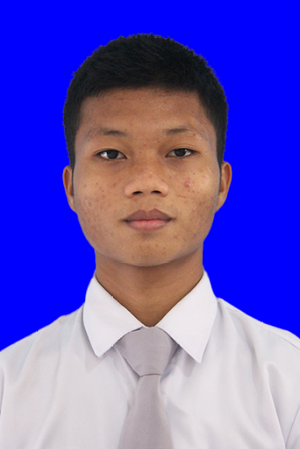
\includegraphics[width=3cm,height=3cm,keepaspectratio]{foto_fikri.png} \\
    \small \textbf{Fikri Rivandi}
\end{minipage}
\hfill
\begin{minipage}{0.7\textwidth}
    \small
    Born in Rokan Hilir, Riau. A student of the Informatics Engineering Study Program, Faculty of Engineering, Universitas Riau, class of 2022. During his studies, he has been active in the Engineering Robotic Club (ERC) UNRI and focuses on Robotics, Computer Vision, Artificial Intelligence, and Embedded Systems. His research focuses on optimizing wheeled soccer robot vision systems using deep learning and Kalman Filter approaches.
\end{minipage}

\vspace{1cm}

\noindent
\begin{minipage}{0.25\textwidth}
    \centering
    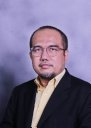
\includegraphics[width=3cm,height=3cm,keepaspectratio]{foto_feri_candra.jpg} \\
    \small \textbf{Feri Candra, S.T., M.T., Ph.D.}
\end{minipage}
\hfill
\begin{minipage}{0.7\textwidth}
    \small
    Lecturer in the Informatics Engineering Study Program, Faculty of Engineering, Universitas Riau. He completed his bachelor's degree at the Institut Sains dan Teknologi Nasional, his master's degree at Universitas Indonesia, and his Ph.D. at Universiti Teknologi Malaysia. He has expertise and research interests in Machine Learning, Computer Vision, Robotics, and the Internet of Things (IoT). He is actively involved as a supervisor for the ERC UNRI robotics team.
\end{minipage}

\end{document}